\chapter{Ion Energy Flux: Definition and Physical Significance}
\label{ch:ief}

The preceding chapters established the plasma sheath as the thin, quasi-neutrality-violating boundary layer through which a bounded plasma communicates with a material surface. This chapter addresses the quantity this monograph takes as its principal diagnostic and design target: the \emph{ion energy flux}, $\Gamma_{E}$, the rate at which kinetic energy carried by ions is delivered per unit area to a plasma-facing surface. Where the particle flux $\Gamma_{\mathrm{i}}$ answers \emph{how many} ions arrive, $\Gamma_E$ answers \emph{how much energy} arrives with them, and this second question governs sputtering yield, etch rate, implantation depth, surface heating, and material damage across plasma-facing applications. We fix definitions and units for particle and energy flux, construct $\Gamma_{E}$ as a moment of the ion velocity distribution function $f_{\mathrm{i}}(v)$, decompose the mean ion energy into directed and thermal parts, describe the ion energy and velocity distribution functions (IEDF/IVDF) carrying this information at a bounding surface, place the ion channel within the full wall power balance, quantify the sensitivity of $\Gamma_{E}$ to $T_{\mathrm{e}}$, $n_{\mathrm{s}}$, and the sheath potential drop, and close by explaining why $\Gamma_{E}$ is not directly measurable -- motivating the reconstruction-based approach of the chapters that follow.

\section{Particle Flux and Energy Flux: Formal Definitions and Units}

\subsection{Particle flux at a bounding surface}

Consider a plasma-facing surface with outward unit normal $\hat{n}$, and let $f_{\mathrm{i}}(\vec r, \vec v, t)$ denote the ion phase-space distribution function, normalized so $n_{\mathrm{i}}(\vec r, t) = \int f_{\mathrm{i}}(\vec r, \vec v, t)\, \mathrm{d}^3 v$ is the local ion number density. The particle flux crossing a surface element is the first velocity moment of $f_{\mathrm{i}}$ projected onto $\hat n$,
\begin{equation}
\Gamma_{\mathrm{i}}(\vec r, t) \;\equiv\; \int_{\mathbb{R}^3} (\vec v \cdot \hat n)\, f_{\mathrm{i}}(\vec r, \vec v, t)\, \mathrm{d}^3 v \;=\; n_{\mathrm{i}}(\vec r,t)\, u_{\mathrm{i}}(\vec r,t),
\label{eq:Gamma-i-def}
\end{equation}
where $u_{\mathrm{i}} \equiv \langle \vec v \cdot \hat n \rangle$ is the mean ion drift speed normal to the surface. Equation~\eqref{eq:Gamma-i-def} has SI units $\si{\per\square\meter\per\second}$ and is the flux measured by a planar probe biased into ion saturation. At the wall, flux conservation through the collisionless sheath links the wall flux to the flux at the sheath edge, $\Gamma_{\mathrm{i}}(\text{wall}) \approx n_{\mathrm{s}} u_{\mathrm{B}}$, with $n_{\mathrm{s}}$ the sheath-edge density and $u_{\mathrm{B}} = \sqrt{T_{\mathrm{e}}/m_{\mathrm{i}}}$ the Bohm speed (temperatures in energy units, $T_{\mathrm{e}} \equiv k_{\mathrm B} T_{\mathrm{e}}$). This near-conservation makes $n_{\mathrm{s}}$, rather than the larger, less accessible wall-adjacent density, the natural anchor point for surface flux calculations -- a role revisited for non-Maxwellian bulk populations in \cite{ref0090}.

\subsection{Energy flux and its physical dimensions}

The energy flux weights each ion's contribution by its kinetic energy $\tfrac{1}{2} m_{\mathrm{i}} v^2$ rather than unity:
\begin{equation}
\Gamma_{E}(\vec r, t) \;\equiv\; \int_{\mathbb{R}^3} \left(\tfrac{1}{2} m_{\mathrm{i}} v^2\right) (\vec v \cdot \hat n)\, f_{\mathrm{i}}(\vec r, \vec v, t)\, \mathrm{d}^3 v.
\label{eq:GammaE-def}
\end{equation}
Dimensionally, $\Gamma_{E}$ is a power per unit area, $\si{\watt\per\square\meter}$, or $\si{\electronvolt\per\square\meter\per\second}$ ($\SI{1}{\electronvolt\per\square\meter\per\second} = \SI{1.602e-19}{\watt\per\square\meter}$). It must be distinguished from the total heat flux $q_{\mathrm{wall}}$, which sums the ion channel with electron, recombination, radiative and secondary-emission contributions (\cref{sec:power-balance}). $\Gamma_{E}$ drives sputtering, ion-assisted etching, and implantation dose-energy products, whereas $q_{\mathrm{wall}}$ governs thermal-management calculations; conflating the two is a common error, flagged in etch-profile modelling \cite{ref0074} and reactive-ion etching of wafers \cite{ref0080}.

\subsection{Distinguishing \texorpdfstring{$\Gamma_{E}$}{Gamma\_E} from related quantities}

Three quantities are frequently confused with $\Gamma_{E}$. First, the ion \emph{energy density} $w_{\mathrm{i}} = \int \tfrac12 m_{\mathrm{i}} v^2 f_{\mathrm{i}}\, \mathrm{d}^3 v$ is volumetric ($\si{\joule\per\cubic\meter}$), not a flux, until convected across a surface via the $(\vec v\cdot\hat n)$ weighting in \cref{eq:GammaE-def}. Second, the \emph{mean ion energy} $\langle E_{\mathrm{i}}\rangle \equiv \Gamma_{E}/\Gamma_{\mathrm{i}}$ is an energy, not a flux, and is what energy-resolved diagnostics such as retarding-field analyzers report directly; $\Gamma_{E}$ requires this multiplied by the co-located particle flux, a combination \cref{sec:observability} shows is rarely available from one measurement. Third, the sheath \emph{heat transmission coefficient} $\gamma_{\mathrm{i}}$, ubiquitous in fusion edge-plasma work \cite{ref0093}, is dimensionless, defined by $\Gamma_{E} \equiv \gamma_{\mathrm{i}} T_{\mathrm{e}} \Gamma_{\mathrm{i}}$; it packages the energetics of \cref{sec:contributions} into one factor, useful for quick estimates but obscuring the dependence on sheath potential made explicit here.

\subsection{Application domains that motivate precise knowledge of \texorpdfstring{$\Gamma_{E}$}{Gamma\_E}}

The stakes attached to an accurate $\Gamma_{E}$ vary across settings. In reactive-ion and plasma-immersion processing, the ion energy flux through a pulsed or biased sheath sets the achievable implantation dose-energy product and treated-layer depth profile. In magnetron physical vapor deposition, particularly its high-power-impulse variant, the angularly resolved ion flux and its energy content control film growth mode, stoichiometry, and microstructure, an effect exploited by the ultra-low-frequency electrical asymmetry effect to tailor the delivered ion energy distribution in biased inductively coupled configurations \cite{ref0106}. In electric propulsion, by contrast, the ion energy flux exhausted from a thruster's acceleration region is the primary quantity of interest, not a boundary condition to minimize, since it is proportional to the product of thrust and exhaust velocity (thrust $\times$ $I_{\mathrm{sp}} g_0$); diagnostics of a Hall-effect thruster plume \cite{ref0114} and reviews of ion thrusters maturing into a mainstream technology \cite{ref0115} underscore how the same quantity carries opposite engineering connotations -- suppressed at a wafer, maximized at a thruster exit. This diversity is why a general, first-principles formulation of $\Gamma_{E}$, rather than case-specific rules, is the right starting point for the reconstruction methodology built later.

\section{The Ion Energy Flux Integral over the Ion Velocity Distribution Function}

\subsection{Moments of \texorpdfstring{$f_{\mathrm{i}}(v)$}{f\_i(v)}: density, flux, and energy flux}

$\Gamma_{E}$ is the energy-weighted first velocity moment of $f_{\mathrm{i}}$, usefully placed within the full moment hierarchy any kinetic or fluid model of the sheath must resolve: the zeroth moment is the density $n_{\mathrm{i}} = \int f_{\mathrm{i}}\, \mathrm{d}^3 v$, the first is $\Gamma_{\mathrm{i}}$, the second yields pressure and kinetic energy density, and $\Gamma_{E}$, built from $v^2 \times v$, is formally a \emph{third}-order moment along $\hat n$. This matters practically: third-order moments are far more sensitive to the high-velocity tail of $f_{\mathrm{i}}$ than the density or flux, so details nearly invisible in $n_{\mathrm{i}}$ or $\Gamma_{\mathrm{i}}$ -- a modest high-energy shoulder from charge exchange or RF sheath modulation -- can dominate $\Gamma_{E}$. This is why fluid closures built only on density and momentum moments routinely fail to capture the ion energy spectrum, motivating fluid models carrying an explicit ion energy-spectrum equation \cite{ref0083} and kinetic treatments resolving the full IVDF at the sheath boundary as a boundary condition in its own right \cite{ref0119}.

For a general non-Maxwellian, drifting, multi-component ion population, no closed-form expression for $\Gamma_{E}$ exists without specifying $f_{\mathrm{i}}$; a useful reference case is the drifting Maxwellian, $f_{\mathrm{i}}(\vec v) = n_{\mathrm{i}} \left(m_{\mathrm{i}}/2\pi T_{\mathrm{i}}\right)^{3/2} \exp\!\left[-m_{\mathrm{i}}(\vec v - \vec u_{\mathrm{i}})^2/2T_{\mathrm{i}}\right]$, for which \cref{eq:GammaE-def} along the drift direction gives the standard fluid closure
\begin{equation}
\Gamma_{E} \;=\; n_{\mathrm{i}} u_{\mathrm{i}} \left(\frac{1}{2} m_{\mathrm{i}} u_{\mathrm{i}}^2 + \frac{5}{2} T_{\mathrm{i}}\right) \;=\; \Gamma_{\mathrm{i}} \left(\frac{1}{2} m_{\mathrm{i}} u_{\mathrm{i}}^2 + \frac{5}{2} T_{\mathrm{i}}\right).
\label{eq:GammaE-drifting-maxwellian}
\end{equation}
The coefficient $5/2$ (not the naive $3/2$) arises because the energy flux carries not only the convected thermal energy $\tfrac32 T_{\mathrm{i}}$ but also the $p\,\mathrm{d}V$ pressure-work term $n_{\mathrm{i}} T_{\mathrm{i}} u_{\mathrm{i}}$ -- an enthalpy-like flux rather than a purely kinetic one. \Cref{eq:GammaE-drifting-maxwellian} is a useful reference precisely because real sheath-edge IVDFs are \emph{not} drifting Maxwellians (truncated by the loss cone into the sheath, often with non-Gaussian tails), so deviations from it are themselves diagnostic of the shape of $f_{\mathrm{i}}$, developed further using non-Maxwellian sheath-formation criteria in \cite{ref0090}.

\subsection{Reduction to a one-dimensional surface-normal problem}

For a planar, unmagnetized (or weakly magnetized, field-aligned) sheath, transverse velocity components decouple from the acceleration along $\hat n$, and it is convenient to use the reduced one-dimensional IVDF,
\begin{equation}
f_{\mathrm{i}}(v_z) \;\equiv\; \int\!\!\int f_{\mathrm{i}}(v_x, v_y, v_z)\, \mathrm{d}v_x\, \mathrm{d}v_y,
\end{equation}
with $z$ along $\hat n$. The particle and energy fluxes at any plane $z$ then collapse to one-dimensional integrals over the outward-directed half of velocity space,
\begin{align}
\Gamma_{\mathrm{i}}(z) &= \int_0^{\infty} v_z\, f_{\mathrm{i}}(v_z)\, \mathrm{d}v_z, \label{eq:Gamma-i-1D}\\
\Gamma_{E}(z) &= \int_0^{\infty} \tfrac{1}{2} m_{\mathrm{i}} v_z^2 \cdot v_z\, f_{\mathrm{i}}(v_z)\, \mathrm{d}v_z. \label{eq:GammaE-1D}
\end{align}
This is the working form used throughout the sheath-diagnostics literature, since energy- and velocity-resolved instruments (retarding-field analyzers, laser-induced fluorescence, mass-resolved energy analyzers) are sensitive to the surface-normal velocity component and report, in effect, $f_{\mathrm{i}}(v_z)$ or its energy-space image.

\subsection{The energy flux in terms of the normalized ion energy distribution function}

It is often more transparent to work in energy space. Define the normalized ion energy distribution function (IEDF) $f_E(E)$ via $E = \tfrac12 m_{\mathrm{i}} v_z^2$, $\mathrm{d}E = m_{\mathrm{i}} v_z\, \mathrm{d}v_z$, such that
\begin{equation}
\int_0^{\infty} f_E(E)\, \mathrm{d}E = 1,
\end{equation}
i.e., $f_E(E)$ is a probability density over arriving-ion energy, independent of flux magnitude. With this normalization, \cref{eq:Gamma-i-1D,eq:GammaE-1D} combine into the compact, central relation
\begin{equation}
\boxed{\;\Gamma_{E} \;=\; \Gamma_{\mathrm{i}} \int_0^{\infty} E\, f_E(E)\, \mathrm{d}E \;=\; \Gamma_{\mathrm{i}}\, \langle E_{\mathrm{i}} \rangle\;}
\label{eq:GammaE-factorized}
\end{equation}
which states that $\Gamma_{E}$ factorizes into particle flux times mean ion energy from the shape-only IEDF. This is the single most important relation in this chapter: it separates \emph{how many} ions arrive, set by $n_{\mathrm{s}}$ and $u_{\mathrm{B}}$, from \emph{how energetic} each is, set by the shape of $f_E(E)$ -- the factorization \cref{sec:observability} shows is the root cause of $\Gamma_{E}$'s non-trivial observability.

\section{Contributions to the Ion Energy Flux: Directed Sheath-Gained Energy and Thermal Energy}
\label{sec:contributions}

\subsection{Ion history from bulk plasma to wall: presheath and sheath}

An ion born deep in the quasi-neutral bulk plasma has, on average, negligible directed energy; its energy at collection is acquired entirely during transit through the presheath and sheath. The presheath is the extended, weakly non-neutral region whose ambipolar field -- sustained by ions and electrons leaving the plasma at equal net rates -- accelerates ions from thermal speeds up to the Bohm speed $u_{\mathrm{B}} = \sqrt{T_{\mathrm{e}}/m_{\mathrm{i}}}$ by the sheath edge; the sheath proper is the much thinner, strongly non-neutral layer, typically several Debye lengths $\lambda_{\mathrm{D}} = \sqrt{\varepsilon_0 T_{\mathrm{e}}/n_{\mathrm{e}} e^2}$, across which most of the wall-directed potential drop occurs and ions are further accelerated essentially collisionlessly, or with partial energy randomization if collisional. Accounting for $\Gamma_{E}$ must therefore track \emph{both} the presheath and sheath potential drops.

\subsection{Decomposition of the mean ion energy}

Combining the presheath and sheath contributions, the mean kinetic energy of an ion arriving at the wall can be written, for a collisionless or weakly collisional sheath, as the sum of three terms:
\begin{equation}
\langle E_{\mathrm{i}} \rangle \;=\; \underbrace{\tfrac{1}{2} m_{\mathrm{i}} u_{\mathrm{B}}^2}_{\text{directed, presheath-acquired}} \;+\; \underbrace{e\,|\Delta\phi_{\mathrm{sh}}|}_{\text{directed, sheath-acquired}} \;+\; \underbrace{\alpha\, T_{\mathrm{i}}}_{\text{thermal spread}},
\label{eq:Ei-decomp}
\end{equation}
where $\Delta\phi_{\mathrm{sh}}$ is the potential drop across the sheath proper, and $\alpha$ is an order-unity factor ($1/2$--$5/2$ depending on the sheath-edge IVDF shape, cf.\ the $5/2\,T_{\mathrm{i}}$ coefficient of \cref{eq:GammaE-drifting-maxwellian}) capturing residual thermal broadening. Since $\tfrac12 m_{\mathrm{i}} u_{\mathrm{B}}^2 = \tfrac12 T_{\mathrm{e}}$, \cref{eq:Ei-decomp} becomes
\begin{equation}
\langle E_{\mathrm{i}} \rangle \;\approx\; \tfrac{1}{2} T_{\mathrm{e}} \;+\; e\,|\Delta\phi_{\mathrm{sh}}| \;+\; \alpha\, T_{\mathrm{i}}.
\label{eq:Ei-decomp-Te}
\end{equation}
For a floating, unbiased wall in a low-temperature electropositive discharge, $|\Delta\phi_{\mathrm{sh}}|$ is of order a few $T_{\mathrm{e}}/e$ (set by the zero-net-current condition); the presheath and sheath contributions are then comparable, and the thermal term is a modest correction for cold ions ($T_{\mathrm{i}} \ll T_{\mathrm{e}}$). For a deliberately or self-consistently biased wall -- DC-biased, RF self-biased, or under active ion-beam/plasma-immersion processing -- $|\Delta\phi_{\mathrm{sh}}|$ can reach tens to hundreds of volts, dwarfing $T_{\mathrm{e}}$, so \cref{eq:Ei-decomp-Te} reduces to $\langle E_{\mathrm{i}}\rangle \approx e|\Delta\phi_{\mathrm{sh}}|$. \Cref{fig:Ei-vs-V} renders this decomposition schematically.

\begin{figure}[htbp]
\centering
\begin{tikzpicture}
\begin{axis}[
 width=0.72\textwidth,
 height=6cm,
 xlabel={Sheath potential drop $|\Delta\phi_{\mathrm{sh}}|$ (\si{\volt})},
 ylabel={Mean ion energy $\langle E_{\mathrm{i}}\rangle$ (\si{\electronvolt})},
 xmin=0, xmax=200,
 ymin=0, ymax=210,
 domain=0:200,
 samples=50,
 axis lines=left,
 thick,
 legend style={draw=black, fill=white, font=\footnotesize, at={(0.03,0.97)}, anchor=north west},
]
\addplot[black, thick] {4.5 + x};
\addlegendentry{$\langle E_{\mathrm i}\rangle = \tfrac12 T_{\mathrm e} + \alpha T_{\mathrm i} + e|\Delta\phi_{\mathrm{sh}}|$}
\addplot[black, dashed] {4.5 + 0*x};
\addlegendentry{Bohm + thermal contribution alone}
\end{axis}
\end{tikzpicture}
\caption{Schematic, analytic illustration of \cref{eq:Ei-decomp-Te}: the mean ion energy delivered to the wall as a function of the sheath potential drop, evaluated for illustrative parameters $T_{\mathrm{e}} = \SI{3}{\electronvolt}$, $\alpha T_{\mathrm i} = \SI{3}{\electronvolt}$ (solid line), compared with the potential-independent presheath-plus-thermal contribution alone (dashed line). This is a plotted analytic function chosen to convey the linear scaling with sheath voltage, not measured or simulated data.}
\label{fig:Ei-vs-V}
\end{figure}

\subsection{The role of collisions in redistributing directed and thermal energy}

The decomposition of \cref{eq:Ei-decomp} assumes an effectively collisionless presheath and sheath, an assumption that fails once the ion-neutral mean free path becomes comparable to, or shorter than, these length scales. Charge-exchange and elastic collisions reduce the net ion flux reaching the wall by scattering ions out of the acceleration trajectory or generating slow ions locally within the sheath \cite{ref0077}, and reshape the energy distribution, converting directed sheath-gained energy into randomized thermal energy and populating a low-energy tail absent in the collisionless limit. In the strongly collisional regime relevant to plasma immersion ion implantation at moderate pressure, the delivered ion energy distribution becomes a convolution of the applied sheath voltage waveform with a collisional broadening kernel that shapes the resulting implantation-depth profile. Such effects act as corrections to, or generalizations of, the three-term decomposition of \cref{eq:Ei-decomp}, entering $\Gamma_{E}$ multiplicatively through \cref{eq:GammaE-factorized} via their effect on the shape of $f_E(E)$.

\subsection{Multiple ion species and the ion energy flux}

Real discharges frequently contain more than one ion species -- different charge states, chemically distinct positive ions, or coexisting positive and negative ions -- and the total ion energy flux is a sum over species,
\begin{equation}
\Gamma_{E}^{\mathrm{tot}} \;=\; \sum_{k} \Gamma_{E,k} \;=\; \sum_{k} \Gamma_{\mathrm{i},k} \langle E_{\mathrm{i},k} \rangle,
\end{equation}
where each species $k$ may reach the sheath edge with a different effective Bohm speed (lighter species can satisfy the generalized multi-species Bohm criterion at a lower fraction of their own Bohm speed) and so contribute disproportionately to $\Gamma_{E}^{\mathrm{tot}}$ relative to its number-density fraction, relevant to multi-species magnetized-sheath energy partitioning in processing tools with mixed feed gases \cite{ref0088}. The single-species framework of \cref{eq:Ei-decomp,eq:GammaE-factorized} generalizes directly, but the total energy flux can differ substantially from a single-species estimate using bulk plasma parameters alone.

\section{Ion Energy and Velocity Distribution Functions at Plasma-Bounded Surfaces}

\subsection{From \texorpdfstring{$f_{\mathrm{i}}(v)$}{f\_i(v)} to the IEDF}

The IVDF $f_{\mathrm{i}}(v)$ and the IEDF $f_E(E)$ are two representations of the same information, related by $E = \tfrac12 m_{\mathrm{i}} v^2$ and its Jacobian, $f_E(E)\, \mathrm{d}E = f_{\mathrm{i}}(v)\, \mathrm{d}v$ with $\mathrm{d}E = m_{\mathrm{i}} v\, \mathrm{d}v$. The IVDF is the more fundamental object kinetically -- it appears natively in the Vlasov equation governing ion evolution through the sheath -- while the IEDF is the representation most directly probed by energy-selective instruments and the one in which \cref{eq:GammaE-factorized} is most transparent. Both are used interchangeably: the IVDF matters whenever directional or angular information is needed (obliquely magnetized sheaths, off-normal incidence), while the IEDF is the natural currency for surface-process modelling, since sputtering yields, reaction probabilities, and implantation ranges are, to leading order, functions of the ion's kinetic energy at impact rather than its full velocity vector.

\subsection{Characteristic shapes of the IEDF: collisionless, RF-modulated, and collisionally broadened}

The shape of $f_E(E)$ at a surface depends strongly on the discharge regime; three archetypes recur. In a collisionless, DC or quasi-DC sheath, ions entering with the narrow, Bohm-speed-centered presheath distribution are accelerated by an essentially fixed potential, producing a relatively narrow IEDF tracking the presheath-plus-sheath energy of \cref{eq:Ei-decomp}, with spread set primarily by $T_{\mathrm{i}}$ and finite transit-time averaging, as targeted by dedicated ion-energy-flux sensors for plasma processing \cite{ref0075}. In an RF-driven sheath, the instantaneous sheath voltage oscillates at the driving frequency and its harmonics, so an ion transiting the sheath samples a time-varying potential; if transit time is short compared to the RF period, an ion "freezes in" a nearly instantaneous sheath voltage, and ions launched at different RF phases arrive with different energies, producing the celebrated \emph{bimodal} (or multi-peaked, at intermediate frequencies) IEDF bracketing the time-averaged sheath voltage; models spanning the full frequency range are developed in \cite{ref0123}. \Cref{fig:iedf-bimodal} sketches this bimodal shape.

\begin{figure}[htbp]
\centering
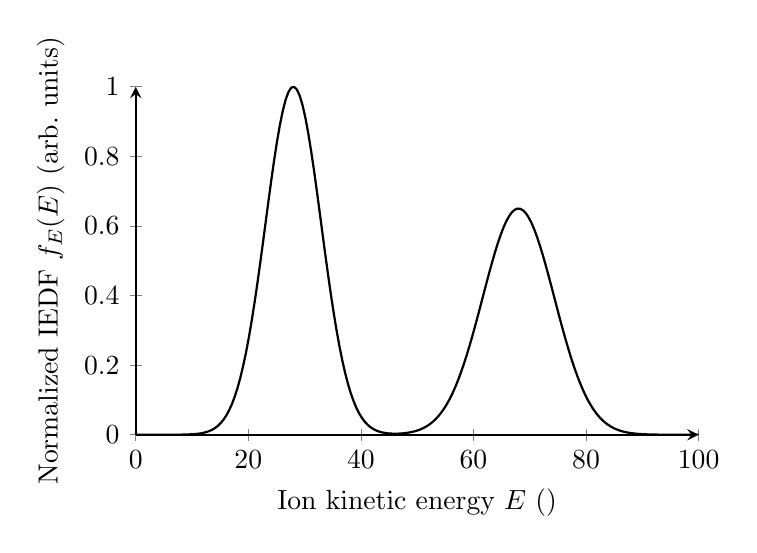
\begin{tikzpicture}
\begin{axis}[
 width=0.72\textwidth,
 height=6cm,
 xlabel={Ion kinetic energy $E$ (\si{\electronvolt})},
 ylabel={Normalized IEDF $f_E(E)$ (arb.\ units)},
 xmin=0, xmax=100,
 ymin=0,
 domain=0:100,
 samples=200,
 axis lines=left,
 thick,
]
\addplot[black, thick] {exp(-((x-28)/7)^2) + 0.65*exp(-((x-68)/9)^2)};
\end{axis}
\end{tikzpicture}
\caption{Schematic, illustrative bimodal ion energy distribution function of the type produced by radio-frequency modulation of the sheath potential drop, drawn as an explicit analytic superposition of two Gaussian components. The curve is not derived from measured or simulated data; it is intended only to convey the characteristic low- and high-energy peak structure discussed in the text.}
\label{fig:iedf-bimodal}
\end{figure}

\subsection{Angular structure, magnetization, and surface-emitted contributions}

Beyond the energy-space shape, the IVDF at a surface retains angular structure relevant to directional sputtering and shadowing in patterned geometries: even in a nominally normal-incidence planar sheath, thermal spread in transverse velocity combined with acceleration only along $\hat n$ narrows the angular spread of incidence as sheath potential increases (larger $e|\Delta\phi_{\mathrm{sh}}|$ collimates the beam), while magnetized sheaths and structured topography broaden it. It is also important to distinguish the IEDF of positive ions launched toward the surface -- this chapter's concern -- from the energy-and-angle distribution of particles \emph{emitted} back into the plasma (sputtered neutrals, backscattered ions, surface-generated negative ions); both matter physically but enter the wall power balance with opposite sign. Further complexity arises in dust-charged discharges or heavy-ion cathode-sheath environments, where the IEDF is shaped jointly by the sheath field and resonant charge-exchange collisions with heavier neutrals.

\subsection{Diagnostic access to the IEDF as a distribution, not merely its mean}

For most surface-process purposes it is not $\langle E_{\mathrm{i}}\rangle$ alone but the full shape of $f_E(E)$ that matters, because sputtering yield and reaction-probability curves are typically nonlinear (threshold-like at low energy, saturating at high energy), so the energy-flux-weighted average of a nonlinear yield function over $f_E(E)$ can differ substantially from the yield evaluated at $\langle E_{\mathrm{i}}\rangle$ alone. This motivates the broader program of "tailoring" the IEDF at plasma electrodes -- shaping the applied waveform to sculpt a desired energy distribution for process optimization -- surveyed comprehensively in \cite{ref0105}.

\section{Power Balance at the Wall: Ion, Electron, Recombination and Radiative Channels}
\label{sec:power-balance}

\subsection{The total power flux to a plasma-facing surface}

$\Gamma_{E}$ is one contribution -- often dominant for processing-relevant ion energies, but never the only one -- to the total power flux $q_{\mathrm{wall}}$ deposited on, or extracted from, a plasma-facing surface:
\begin{equation}
q_{\mathrm{wall}} \;=\; \Gamma_{E,\mathrm{ion}} \;+\; \Gamma_{E,\mathrm{electron}} \;+\; \Gamma_{\mathrm{i}}\, \varepsilon_{\mathrm{recomb}} \;-\; \Gamma_{\mathrm{see}}\, E_{\mathrm{see}} \;+\; q_{\mathrm{rad}},
\label{eq:power-balance-total}
\end{equation}
where the five terms are, respectively, the ion kinetic-plus-potential channel of this chapter, the electron thermal-flux channel, the energy released when an arriving ion recombines at the wall (recovering ionization energy $\varepsilon_{\mathrm{recomb}}$ as heat), the energy carried \emph{away} by secondary/backscattered electrons emitted with characteristic energy $E_{\mathrm{see}}$ at rate $\Gamma_{\mathrm{see}}$ (a loss term), and any net radiative flux $q_{\mathrm{rad}}$. Rigorous reactor-scale accounting of this balance, with ion and electron channels expressed through heat-transmission coefficients coupled to the confined-plasma energy balance, is treated in \cite{ref0093}, while device-specific total heat-flux measurements from ion bombardment of a wafer in an inductively coupled etch tool illustrate the practical side \cite{ref0080}. \Cref{tab:power-channels} summarizes the five channels.

\begin{table}[htbp]
\centering
\caption{Principal channels contributing to the total power flux deposited on a plasma-facing surface, \cref{eq:power-balance-total}. The ion energy flux $\Gamma_{E}$ that is the subject of this chapter constitutes only the first row; the remaining channels must be independently characterized, or subtracted, to isolate it from a total heat-load measurement.}
\label{tab:power-channels}
\begin{tabular}{@{}p{3.4cm}p{6.0cm}p{4.4cm}@{}}
\toprule
Channel & Physical origin & Sign / scaling \\
\midrule
Ion kinetic + potential ($\Gamma_{E,\mathrm{ion}}$) & Presheath (Bohm) and sheath acceleration plus thermal spread, \cref{eq:Ei-decomp-Te} & $+$; $\propto n_{\mathrm{s}} u_{\mathrm{B}}\, e|\Delta\phi_{\mathrm{sh}}|$ \\
Electron thermal ($\Gamma_{E,\mathrm{electron}}$) & High-energy tail of the (truncated) electron distribution reaching the wall & $+$; $\propto n_{\mathrm{s}} \bar v_{\mathrm{e}} T_{\mathrm{e}}$ \\
Recombination & Ionization energy released on neutralization at the surface & $+$; $\propto \Gamma_{\mathrm{i}}\,\varepsilon_{\mathrm{recomb}}$ \\
Secondary/backscattered emission & Energy carried away by electrons or ions ejected from the surface & $-$; $\propto \Gamma_{\mathrm{i}}\, \gamma_{\mathrm{se}}\, E_{\mathrm{see}}$ \\
Radiative & Photon absorption/emission at or near the surface & $\pm$; typically subdominant at low pressure, potentially significant in dense or strongly radiating plasmas \\
\bottomrule
\end{tabular}
\end{table}

\subsection{The ion channel and the sheath heat transmission coefficient}

Formally, the ion channel of \cref{eq:power-balance-total} is exactly $\Gamma_{E}$ as constructed in \cref{sec:contributions,eq:GammaE-factorized}, commonly packaged as $\Gamma_{E,\mathrm{ion}} = \gamma_{\mathrm{i}} T_{\mathrm{e}} \Gamma_{\mathrm{i}}$, defining $\gamma_{\mathrm{i}} \equiv \langle E_{\mathrm{i}}\rangle / T_{\mathrm{e}}$. For a floating wall with negligible bias, $\gamma_{\mathrm{i}}$ typically falls in the range $2$--$3$, reflecting \cref{eq:Ei-decomp-Te} at the floating potential; for actively biased surfaces, $\gamma_{\mathrm{i}}$ scales linearly with bias voltage over $T_{\mathrm{e}}$, so $\gamma_{\mathrm{i}} \gg 1$ is routine with substantial substrate bias. Data-driven approaches discovering closed-form heat-flux closures directly from kinetic or particle-in-cell simulation data offer an independent cross-check on closures of this kind \cite{ref0101}.

\subsection{The electron channel}

Electrons reaching the wall are drawn from the high-energy tail of the electron distribution with sufficient normal velocity to overcome the retarding sheath potential; for a floating or negatively biased wall this is an exponentially suppressed fraction of the bulk population, but because the electron thermal speed $\bar v_{\mathrm{e}} = \sqrt{8T_{\mathrm{e}}/\pi m_{\mathrm{e}}}$ is roughly $\sqrt{m_{\mathrm{i}}/m_{\mathrm{e}}}$ times the ion Bohm speed, the electron channel remains a significant, and for near-floating walls comparable, contributor to $q_{\mathrm{wall}}$. The electron and ion channels are not independent: ambipolarity directly determines $\Delta\phi_{\mathrm{sh}}$ in \cref{eq:Ei-decomp-Te}, so any change in the electron energy distribution alters the electron channel directly and the ion channel indirectly through the self-consistent sheath voltage.

\subsection{Recombination and secondary-emission channels}

The recombination channel is often neglected in low-temperature processing-plasma power balances since the ionization energy of common process gases is comparable to, or smaller than, typical sheath-acquired ion energies at moderate bias; it becomes non-negligible in high-density or high-charge-state plasmas and is retained in comprehensive reactor-scale balances \cite{ref0093}. The secondary-emission channel is more consequential: ion-induced (and, for energetic populations, electron-induced) secondary electron emission removes energy from the surface at a rate proportional to the incident flux and the secondary emission yield $\gamma_{\mathrm{se}}$, and because emitted secondaries are accelerated back out through the sheath potential, monitoring their energy and flux provides an indirect but accessible proxy for the incident ion flux, exploited in plasma-immersion implantation diagnostics tracking sheath-accelerated secondary electrons \cite{ref0078}.

\section{Sensitivity of the Ion Energy Flux to \texorpdfstring{$T_{\mathrm{e}}$}{Te}, \texorpdfstring{$n_{\mathrm{s}}$}{ns}, and Sheath Potential}

\subsection{Functional form and scaling}

Combining \cref{eq:GammaE-factorized} with the flux and mean-energy expressions of \cref{sec:contributions} gives an explicit functional form for $\Gamma_{E}$ in terms of the three controlling parameters emphasized throughout this monograph:
\begin{equation}
\Gamma_{E} \;=\; n_{\mathrm{s}} \sqrt{\frac{T_{\mathrm{e}}}{m_{\mathrm{i}}}} \left(\tfrac{1}{2} T_{\mathrm{e}} + e|\Delta\phi_{\mathrm{sh}}| + \alpha T_{\mathrm{i}}\right).
\label{eq:GammaE-scaling}
\end{equation}
Three structural features deserve emphasis. First, $\Gamma_{E}$ is exactly linear in $n_{\mathrm{s}}$, entering only through the flux prefactor -- a direct, testable consequence of \cref{eq:GammaE-factorized}. Second, $T_{\mathrm{e}}$ enters twice -- through the Bohm-speed prefactor $\sqrt{T_{\mathrm{e}}/m_{\mathrm{i}}}$ and the $\tfrac12 T_{\mathrm{e}}$ presheath-energy term -- so even at fixed sheath potential, $\Gamma_{E}$ is more sensitive to $T_{\mathrm{e}}$ than to $n_{\mathrm{s}}$ whenever the presheath term is not negligible compared with $e|\Delta\phi_{\mathrm{sh}}|$. Third, $\Delta\phi_{\mathrm{sh}}$ enters only inside the energy bracket, linearly, but is frequently not independent: at a floating wall it is set by $T_{\mathrm{e}}$ through ambipolarity, while at a biased wall it may be set externally or self-consistently by discharge power, geometry, and frequency.

\subsection{Logarithmic sensitivity coefficients}

It is convenient to express the sensitivity of $\Gamma_{E}$ to each parameter $X \in \{n_{\mathrm{s}}, T_{\mathrm{e}}, |\Delta\phi_{\mathrm{sh}}|\}$ through the logarithmic derivative $\partial \ln \Gamma_{E} / \partial \ln X$, useful for propagating measurement uncertainties. From \cref{eq:GammaE-scaling}, holding the other two parameters fixed,
\begin{align}
\frac{\partial \ln \Gamma_{E}}{\partial \ln n_{\mathrm{s}}} &= 1, \label{eq:sens-ns}\\[4pt]
\frac{\partial \ln \Gamma_{E}}{\partial \ln |\Delta\phi_{\mathrm{sh}}|} &= \frac{e|\Delta\phi_{\mathrm{sh}}|}{\tfrac12 T_{\mathrm{e}} + e|\Delta\phi_{\mathrm{sh}}| + \alpha T_{\mathrm{i}}}, \label{eq:sens-V}\\[4pt]
\frac{\partial \ln \Gamma_{E}}{\partial \ln T_{\mathrm{e}}} &= \frac{1}{2} + \frac{\tfrac12 T_{\mathrm{e}}}{\tfrac12 T_{\mathrm{e}} + e|\Delta\phi_{\mathrm{sh}}| + \alpha T_{\mathrm{i}}}, \label{eq:sens-Te}
\end{align}
where \cref{eq:sens-ns} is exact for all regimes, while \cref{eq:sens-V,eq:sens-Te} interpolate depending on the relative size of $e|\Delta\phi_{\mathrm{sh}}|$ and $T_{\mathrm{e}}$. In the strongly biased limit ($e|\Delta\phi_{\mathrm{sh}}| \gg T_{\mathrm{e}}$), \cref{eq:sens-V} tends to unity and \cref{eq:sens-Te} to $1/2$: $\Gamma_{E}$ scales linearly with bias voltage and as $\sqrt{T_{\mathrm{e}}}$ once the sheath energy term dominates. In the near-floating limit ($e|\Delta\phi_{\mathrm{sh}}| \sim T_{\mathrm{e}}$, with $\Delta\phi_{\mathrm{sh}} \propto T_{\mathrm{e}}$ through ambipolarity), the two contributions to $T_{\mathrm{e}}$-sensitivity add and the effective exponent rises toward $3/2$, so $\Gamma_{E}$ at a floating or lightly biased wall is considerably more sensitive to electron-temperature uncertainty than the naive $1/2$-power Bohm-flux scaling suggests. Non-Maxwellian electron populations reshape these Maxwellian-derived exponents.

\subsection{Regime dependence: floating, strongly biased, and RF self-biased walls}

\Cref{tab:sensitivity} collects illustrative sensitivity exponents for three representative regimes, from the limiting forms of \cref{eq:sens-ns,eq:sens-V,eq:sens-Te}. The magnetized-sheath case adds a further layer of sensitivity beyond \cref{eq:GammaE-scaling}, since the effective ion acceleration and delivered kinetic energy also depend on magnetic-field strength and obliquity \cite{ref0088}. A further important regime is a plasma at floating potential on a topographically or electrically patterned surface, where the local sheath structure -- and hence local $\Delta\phi_{\mathrm{sh}}$ and $\Gamma_{E}$ -- can vary substantially across the surface even with uniform bulk $n_{\mathrm{s}}$ and $T_{\mathrm{e}}$, a reminder that this sensitivity analysis strictly applies only locally.

\begin{table}[htbp]
\centering
\caption{Illustrative logarithmic sensitivity exponents $\partial \ln \Gamma_{E} / \partial \ln X$ of the ion energy flux to the sheath-edge density, electron temperature, and sheath potential drop, in three representative bias regimes, derived from the limiting forms of \cref{eq:sens-ns,eq:sens-V,eq:sens-Te}. The tabulated values are schematic, illustrating the analytic scaling rather than fitted results from measured or simulated discharges.}
\label{tab:sensitivity}
\begin{tabular}{@{}lccc@{}}
\toprule
Regime & $n_{\mathrm{s}}$ & $T_{\mathrm{e}}$ & $|\Delta\phi_{\mathrm{sh}}|$ \\
\midrule
Floating wall ($e|\Delta\phi_{\mathrm{sh}}| \propto T_{\mathrm{e}}$) & $1$ & $\approx 3/2$ & not independent of $T_{\mathrm{e}}$ \\
Strongly biased wall ($e|\Delta\phi_{\mathrm{sh}}| \gg T_{\mathrm{e}}$, external bias) & $1$ & $\approx 1/2$ & $\approx 1$ \\
RF self-bias (moderate collisionality) & $1$ & $1/2$--$1$ & $\approx 1$ \\
\bottomrule
\end{tabular}
\end{table}

\subsection{Propagation of measurement uncertainty into \texorpdfstring{$\Gamma_{E}$}{Gamma\_E}}

The sensitivity coefficients above propagate independent measurement uncertainties in $n_{\mathrm{s}}$, $T_{\mathrm{e}}$, and $\Delta\phi_{\mathrm{sh}}$ into an uncertainty estimate on the reconstructed $\Gamma_{E}$. Treating the three as uncorrelated, the fractional uncertainty follows the standard first-order propagation formula
\begin{equation}
\left(\frac{\delta \Gamma_{E}}{\Gamma_{E}}\right)^2 \;\approx\; \left(\frac{\partial \ln \Gamma_{E}}{\partial \ln n_{\mathrm{s}}}\right)^{2} \left(\frac{\delta n_{\mathrm{s}}}{n_{\mathrm{s}}}\right)^{2} + \left(\frac{\partial \ln \Gamma_{E}}{\partial \ln T_{\mathrm{e}}}\right)^{2} \left(\frac{\delta T_{\mathrm{e}}}{T_{\mathrm{e}}}\right)^{2} + \left(\frac{\partial \ln \Gamma_{E}}{\partial \ln |\Delta\phi_{\mathrm{sh}}|}\right)^{2} \left(\frac{\delta |\Delta\phi_{\mathrm{sh}}|}{|\Delta\phi_{\mathrm{sh}}|}\right)^{2}.
\label{ch04-eq:error-propagation}
\end{equation}
Because the exponents are all of order unity across every regime in \cref{tab:sensitivity}, \cref{ch04-eq:error-propagation} shows a fractional uncertainty on any one input parameter propagates into $\Gamma_{E}$ with roughly comparable, not strongly amplified or suppressed, weight. This is reassuring but not trivial: the dominant source of uncertainty in any practical reconstruction is the accuracy of the underlying diagnostics for $n_{\mathrm{s}}$, $T_{\mathrm{e}}$, and $\Delta\phi_{\mathrm{sh}}$ individually, not any intrinsic amplification in the combining expression. In practice, the electron-temperature term is usually the largest contributor to $\delta \Gamma_{E}/\Gamma_{E}$, both because $T_{\mathrm{e}}$ is often the least precisely determined of the three (nonlinear diagnostic inference, sensitivity to non-Maxwellian departures) and because its sensitivity exponent is largest near the floating-wall limit -- motivating the emphasis, in later diagnostic chapters, on obtaining $T_{\mathrm{e}}$ from methods insensitive to assumptions about the electron energy distribution function's shape.

\section{Why the Ion Energy Flux Is Not Directly Measurable}
\label{sec:observability}

\subsection{The instrumental gap between flux and energy}

The factorization $\Gamma_{E} = \Gamma_{\mathrm{i}} \langle E_{\mathrm{i}}\rangle$ is not merely a mathematical convenience; it exposes the central practical obstacle to measuring $\Gamma_{E}$ directly. Instruments that measure particle flux with high fidelity -- planar Langmuir probes in ion saturation, ion-collecting Faraday cups -- are, by design, energy-blind: they count ions regardless of individual kinetic energy, so their output is proportional to $\Gamma_{\mathrm{i}}$ alone. Conversely, instruments that resolve ion energy with high fidelity -- retarding-field analyzers, electrostatic/magnetic energy analyzers, velocity-resolved optics -- report the \emph{shape} of $f_E(E)$ but, in almost every practical implementation, only up to a poorly calibrated absolute normalization: grid transmission factors, finite acceptance angles, space-charge effects, and sheath perturbation by the analyzer's own biased aperture corrupt the absolute count rate while leaving the relative energy distribution comparatively unaffected. No single, standard instrument returns the product $\Gamma_{E} = \Gamma_{\mathrm{i}} \langle E_{\mathrm{i}} \rangle$ directly; $\Gamma_{E}$ must be reconstructed by combining an absolutely calibrated flux measurement with a separately obtained, shape-only energy distribution.

\subsection{Calorimetric and dedicated sensor approaches}

An alternative route is calorimetric: measure the total power deposited on a small sensor embedded in, or substituting for, the wall, via thermal balance. This measures $q_{\mathrm{wall}}$ of \cref{eq:power-balance-total} directly and with good absolute accuracy, but $q_{\mathrm{wall}}$ conflates the ion channel with electron, recombination, and secondary-emission channels; isolating $\Gamma_{E,\mathrm{ion}}$ requires either biasing the sensor to reject electrons (itself perturbing the local sheath) or independently characterizing and subtracting the non-ion channels. Purpose-built ion energy flux sensors combining a biased collector with filtering to suppress electron and secondary-electron contributions have been developed for plasma-processing applications \cite{ref0075}; complementary, less invasive approaches infer incident ion flux by monitoring sheath-accelerated secondary electrons ejected back into the plasma, which scale with, but are not identical to, the primary ion flux and require an assumed or independently measured secondary-emission yield to invert \cite{ref0078}.

\subsection{Energy-resolved and velocity-resolved diagnostics}

Retarding-field energy analyzers remain the workhorse for measuring $f_E(E)$ near a plasma-facing surface, but reliability depends on operating in a regime where the analyzer's own sheath, grid transparency, and space-charge limit do not distort the measured spectrum -- particularly through RF- or pulse-biased sheaths, where the instantaneous sheath potential varies within the ion transit time itself. Complementary, minimally invasive velocity-resolved measurements of the IVDF are obtained via laser-induced fluorescence, probing a localized velocity-space population without a material collector immersed in the plasma. Because raw fluorescence spectra are themselves an indirect, convolved measurement of the underlying IVDF (folding in lineshape broadening, laser linewidth, detection noise), extracting a reliable IVDF -- and reliable $\langle E_{\mathrm{i}}\rangle$ -- generally requires a further inversion step, and absolute normalization to an independently calibrated flux remains a separate, non-trivial step even once the IVDF shape is well measured.

\subsection{Cross-validation across independent reconstruction routes}

A further consequence of the two-factor structure of \cref{eq:GammaE-factorized} is that it enables cross-validation between independent reconstruction routes even absent any single instrument capable of measuring $\Gamma_{E}$ directly. If $\Gamma_{\mathrm{i}}$ is obtained from a Langmuir-probe estimate of $n_{\mathrm{s}}$ combined with the Bohm-speed expression, and $\langle E_{\mathrm{i}}\rangle$ from a retarding-field analyzer, the resulting $\Gamma_{E}$ can be checked against an independent calorimetric estimate (once the non-ion channels of \cref{eq:power-balance-total} are subtracted), or against an analytic sheath-model estimate from \cref{eq:GammaE-scaling} at independently measured $n_{\mathrm{s}}$, $T_{\mathrm{e}}$, and $\Delta\phi_{\mathrm{sh}}$. Agreement between two or more such routes, each with different systematic errors, provides validation no single measurement could offer alone; disagreement is itself diagnostically informative, typically pointing to a specific failure -- unaccounted collisional broadening of the IED, an underestimated secondary-emission yield, or a departure from the collisionless Bohm-flux assumption used to convert $n_{\mathrm{s}}$ into $\Gamma_{\mathrm{i}}$. This cross-validation logic is what allows a reconstructed $\Gamma_{E}$ to carry a defensible uncertainty budget of the kind built from \cref{ch04-eq:error-propagation}, rather than one inherited uncritically from a single instrument's stated precision.

\subsection{Reconstruction as the practical route to \texorpdfstring{$\Gamma_{E}$}{Gamma\_E}}

Taken together, these instrumental limitations lead to a single conclusion: $\Gamma_{E}$ is, in essentially all practical laboratory and industrial settings, an \emph{inferred} rather than a \emph{directly measured} quantity. It is obtained by combining (i) an absolutely calibrated, energy-blind measurement or model of $\Gamma_{\mathrm{i}}$ (from probe theory, a validated discharge model, or $n_{\mathrm{s}} u_{\mathrm{B}}$ once $n_{\mathrm{s}}$ and $T_{\mathrm{e}}$ are known), with (ii) a shape-only, relatively calibrated measurement or model of $\langle E_{\mathrm{i}}\rangle$ (from an energy analyzer, velocity-resolved optics, or a sheath model such as \cref{eq:Ei-decomp-Te} once $\Delta\phi_{\mathrm{sh}}$ is known), multiplied according to \cref{eq:GammaE-factorized}. This reconstruction can also proceed in reverse: given a measured IED and a constrained sheath model, one can work backward to reconstruct the time-averaged sheath potential profile itself, using the ion population as an in-situ probe of the field structure that produced it -- underlying also why rare, high-energy events in $f_E(E)$ can dominate nonlinear surface-response functions while contributing negligibly to $\Gamma_{\mathrm{i}}$ itself \cite{ref0096}. It is this necessarily indirect, multi-diagnostic, model-mediated character of $\Gamma_{E}$ -- not any fundamental inaccessibility of the underlying physics -- that motivates the reconstruction methodology developed in the chapters that follow, where $n_{\mathrm{s}}$, $T_{\mathrm{e}}$, and $\Delta\phi_{\mathrm{sh}}$ are each obtained from complementary, individually validated diagnostics and combined through \cref{eq:GammaE-scaling} into a self-consistent estimate of the ion energy flux delivered to the surface of interest.

\section{Summary}

This chapter formalized $\Gamma_{E}$ as the energy-weighted (third-order) velocity moment of the ion distribution function crossing a plasma-bounded surface, establishing the central factorization $\Gamma_{E} = \Gamma_{\mathrm{i}} \langle E_{\mathrm{i}} \rangle$ separating particle-flux and mean-energy contributions. The mean ion energy was decomposed into a Bohm/presheath-acquired directed term ($\tfrac12 T_{\mathrm{e}}$), a sheath-acquired directed term ($e|\Delta\phi_{\mathrm{sh}}|$), and a thermal spread term ($\alpha T_{\mathrm{i}}$), whose relative weight sets the characteristic IEDF shape -- narrow and quasi-monoenergetic collisionlessly, bimodal under RF modulation, collisionally broadened at elevated pressure. The ion channel was placed within the full wall power balance alongside electron, recombination, and secondary-emission contributions, and the sensitivity of $\Gamma_{E}$ to $n_{\mathrm{s}}$, $T_{\mathrm{e}}$, and $\Delta\phi_{\mathrm{sh}}$ was quantified through logarithmic-derivative expressions interpolating between near-floating and strongly biased regimes. Finally, the chapter argued, on instrumental and physical grounds, that $\Gamma_{E}$ is not accessible to any single standard diagnostic but must be reconstructed from separately calibrated flux and energy-distribution information -- motivating the multi-diagnostic reconstruction framework developed in the chapters that follow.
